\outlineSubframe{Allgemeines}
\begin{frame}{Collections}{Was genau ist das eigentlich? (Vgl. \cite{collection1}}
    \begin{itemize}[<+->]
        \item Kann sowohl bezeichnen:
        \begin{itemize}
            \item Das Collections \textit{Framework}
            \item Das Collections \textit{Interface} (Als Teil des Collection Frameworks)
        \end{itemize}
        \item Collections sind grundlegend:
        \begin{itemize}
            \item Datenstrukturen um eine Gruppe von Elementen zu speichern...
            \item ...und zu manipulieren
        \end{itemize}
        \item Das Collections Framework ist eine Zusammenfassung aus Klassen, Interfaces und Algorithmen
    \end{itemize}
\end{frame}

\begin{frame}{Collections Framework}{Übersicht}
    \begin{figure}
    \centering
    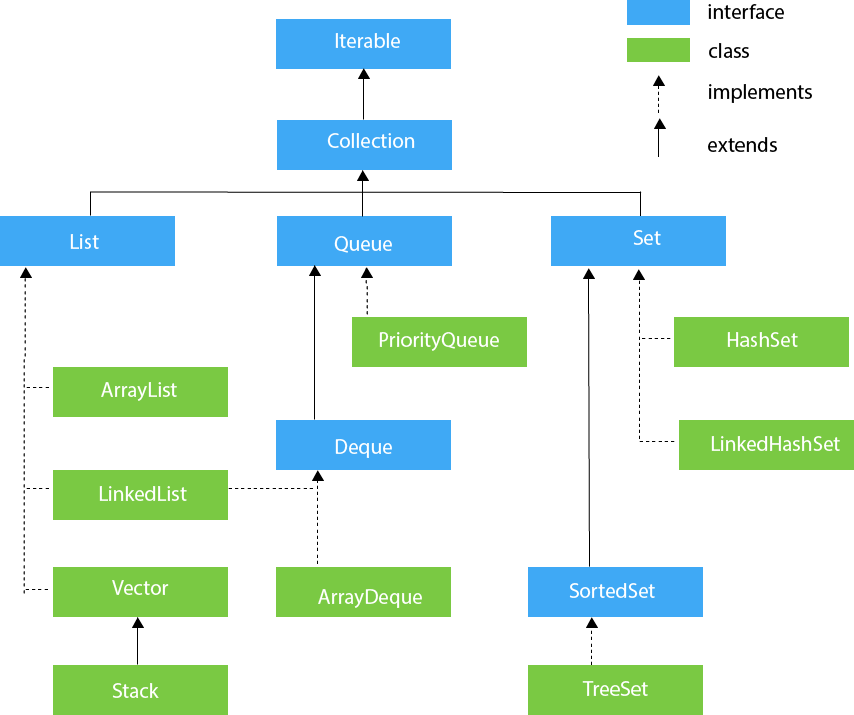
\includegraphics[height=5cm]{graph/java-collection-hierarchy}
    \caption{Quelle: \cite{collection1}}
    \end{figure}
\end{frame}

\begin{frame}{Collections Framework}{Übersicht}
    \begin{itemize}[<+->]
        \item Bestes Anwendungsbeispiel für Generics
        \begin{itemize}
            \item Listen sind für \textbf{alle} Klassen verwendbar...
            \item ...ohne, dass irgendwelche Änderungen vorgenommen werden müssen
        \end{itemize}
        \item C++ Äquivalent: STL Containers
        \begin{itemize}
            \item Seit C++11 teil des Standards
            \item Umfasst einige Datenstrukturen, die Collections nicht haben
        \end{itemize}
    \end{itemize}
\end{frame}

\outlineSubframe{Interfaces\&Klassen}
\begin{frame}{Collection}{Der Grundstein (Vgl. \cite{orac:collection}}
    \begin{itemize}[<+->]
        \item Grundlegendes Interface für alle Subinterfaces und Klassen
        \item Definiert grundlegende Methoden zum:
        \begin{itemize}
            \item Hinzufügen...
            \item Entfernen...
            \item Vergleichen...
            \item Zählen...
            \item ...von Elementen
        \end{itemize}
        \item Noch keine (direkte) Methode zum \textit{lesen} von Elementen
    \end{itemize}
\end{frame}

\begin{frame}{List}{}
    \begin{itemize}[<+->]
        \item Grundsätzliche Struktur für Listen von Elementen
        \item Keine Einschränkung der enthaltenen Elemente
        \item Erlaubt random access von Elementen
        \item Reihenfolge der Elemente wird beibehalten
        \begin{itemize}
            \item Heißt, Elemente liegen in der Reihenfolge vor, wie sie hinzugefügt wurden
            \item Sofern die Liste nicht anderweitig modifiziert wurde (Sortieren o.Ä.)
        \end{itemize}
    \end{itemize}
\end{frame}

\begin{frame}{ArrayList}{Implementierung des List Interfaces}
    \begin{itemize}[<+->]
        \item Daten werden in dynamsichen Array gespeichert
        \item Größe von diesem wird nach Bedarf (im Hintergrund oder auf Anfrage) angepasst
        \item Sehr ähnlich zur \texttt{Vector} Implementierung...
        \begin{itemize}
            \item Jedoch nicht synchronisiert...
            \item ...und deshalb nicht für multithreaded Anwendungen geeignet
        \end{itemize}
    \end{itemize}
\end{frame}

\begin{frame}{LinkedList}{Implementierung des List Interfaces}
    \begin{itemize}[<+->]
        \item Daten werden als Double-Linked-List gespeichert
        \item Ermöglicht Zugriff von beiden "`Enden"' der Liste
        \item Implementiert sowohl \texttt{List} Interface, als auch \texttt{Deque} Interface
        \item Ähnlich wie \texttt{ArrayList}: Nicht thread-safe
    \end{itemize}
\end{frame}

\begin{frame}{Vector}{}
    \begin{itemize}[<+->]
        \item Existierte schon vor dem \texttt{Collections} Framework
        \item Wurde in dieses aufgenommen
        \item Im Grunde ähnlich wie \texttt{ArrayList}
        \item Aber: Thread-Safe
    \end{itemize}
\end{frame}


\begin{frame}{Queue}
    \begin{itemize}[<+->]
        \item Repräsentiert eine "`Warteschlange"'
        \item Für Elemente gilt \textbf{FIFO}:
        \begin{itemize}
            \item \textbf{F}irst \textbf{I}n \textbf{F}irst \textbf{O}ut
            \item Nur Zugriff auf vorderstes Element
        \end{itemize}
        \item Reihenfolge der Elemente nicht unbedingt beibehalten
        \begin{itemize}
            \item \texttt{PriorityQueue} sortiert Element automatisch
        \end{itemize}
    \end{itemize}
\end{frame}

\begin{frame}{Deque}
    \begin{itemize}[<+->]
        \item \textbf{D}ouble \textbf{e}nded \textbf{Que}ue
        \item Subklasse von \texttt{Queue}
        \item Erlaubt jedoch Zugriff auf erstes und letztes Element der Liste
        \item Somit Verwendung auch zB. als \textbf{LIFO} Liste
        \begin{itemize}
            \item \textbf{L}ast \textbf{I}n \textbf{F}irst \textbf{O}ut
        \end{itemize}
    \end{itemize}
\end{frame}

\begin{frame}{Set}
    \begin{itemize}
        \item Vergleichbar mit einer mathematischen Menge
        \begin{itemize}
            \item Jedes Element kann genau einmal vorkommen
        \end{itemize}
        \item Je nach Implementierung...
        \begin{itemize}
            \item ...wird die Reihenfolge der Daten beibehalten
            \item ...werden die Daten strukturiert
        \end{itemize}
    \end{itemize}
\end{frame}

\begin{frame}{Map}{Die Collection die keine ist}
    \begin{itemize}
        \item Gehört mit zum Collections Framework
        \item Erbt jedoch \textbf{nicht} vom Collections Interface
        \item Implementiert jedoch sog. \textit{collection-views}
        \item Speichert eine Gruppe an \textit{KeyValuePairs}
        \begin{itemize}
            \item Wobei hier die \textit{Keys} nicht mehrfach vorkommen
        \end{itemize}
        \item Je nach Implementierung sortiert oder nicht
    \end{itemize}
    
    Vgl. \cite{orac:map}, \cite{map1}
\end{frame}